\title{Enumerative geometry of K3 surfaces}
\author{\textit{Based on a lecture series by }Qaasim Shafi.}
\date{December 2023}
\maketitle

\newcommand{\Jac}{\mathop{\mathcal{J\kern -0.5pt a\kern -0.5pt c\kern -1pt}}}
\newcommand{\IJac}{\mathop{I\mathcal{J\kern -0.5pt a\kern -0.5pt c\kern -1pt}}}
\newcommand{\Moduli}{\ensuremath{\mathscr{M}}}

Enumerative geometry starts off from the very classical problem of counting
lines in a variety. We follow two parallel stories --- first for a K3 surface, and
then for projective space with additional boundary conditions. The count of
rational curves on a K3 surface is given by the Yau--Zaslow formula in terms of
a modular form, and the counts of higher genus curves is determined by the
counts of rational curves. Abstracting the intersection-theoretic arguments
shows that in fact we often do not count curves, but instead get `generalised
curve counts' called \textit{Gromov--Witten invariants} which are better behaved
under deformations. This deformation invariance is exploited when there are
imposed tangency conditions on the count, to degenerate the variety and reduce
the problem to a combinatorial count. Throughout, we see how intuition from
the K3 count feeds into this general theory, in particular we are able to
`guess' the relationship between counts of rational curves and those of higher
genus curves.

\subsection{About} This course on enumerative geometry was a part of a Winter
School for early career researchers, organised by the UK Algebraic
Geometry Network. The lectures were delivered in-person in the University of
Warwick, and were transcribed by Parth Shimpi. 
Parts of this course are based on a lecture by Rahul Pandharipande
(\url{https://www.youtube.com/watch?v=TBoonBCDRa8}). These notes have undergone
several amendments and are not a verbatim recall of the lectures, therefore
discretion is advised when using them. They are available online at
\url{https://pas201.user.srcf.net/documents/2023-ukag-enum-geom.pdf}.

All errors and corrections should be communicated to by email to
\url{pas201@srcf.net}.


\section{Rational curves on K3 surfaces}
How many lines on a smooth hypersurface \(X\subset \mathbb{P}^3\) of degree
\(d\)? If \(d=2\), then the surface is a quadric (isomorphic to
\(\mathbb{P}^1\times \mathbb{P}^1\)) and is covered by lines --- in particular
there are two sets transverse rulings. If \(d=3\), then the surface is cubic
and famously contains 27 lines --- we have lost almost all the lines! More
generally, all surfaces of degree \(d\leq 3\) are rational and hence contain
plenty of rational curves. On the other hand if \(d\geq 5\), it can be
shown that \(X\) has no lines and no rational curves of any degree.

What about \(d=4\)? This case plays a transitional role similar to the one
played by elliptic curves for the arithmetic problem of counting
\(\mathbb{Q}\)-points on curves. Suppose \(X\) is defined by a degree \(4\)
polynomial \(f_4\). By definition, a degree \(e\) rational curve in \(X\) is a
map \(\mathbb{P}^1\to X\) defined by three homogeneous polynomials
\(p_0,\ldots,p_3\) of degree \(e\) satisfying \(f_4(p_0,\ldots,p_3)=0\). Hence we may
try to na\"ively count the dimension of the space of degree \(e\) rational
curves in \(X\) as
\[
    \overbracket{(
        \underbrace{4e+4}_\text{[Each \(p_i\) has \(e+1\) coefficients]}
        -\underbrace{1}_\text{[Projectivise]}
        -\underbrace{3}_{[\dim\text{Aut}\mathbb{P}^1]})}
    ^{\dim\{\text{degree \(e\) rational curves in \(\mathbb{P}^1\)}\}}
    -\overbracket{
        (\underbrace{4e+1}_\text{[A degree \(4e\) homogeneous polynomial
        should identically vanish]})}
    ^{\dim\{\text{constraints to lie on \(X\)}\}}
    =-1.
\]
Thus the dimension count suggests there are no rational curves. However, one can
very explicitly find rational curves by showing that \(X\) intersects a
tri-tangent plane in a degree \(4\) curve with three nodes, i.e.\ a rational
curve! Thus some of the constraints in our dimension count do not intersect transversely.

\subsection{What makes degree \(4\) interesting?} It is because quartic surfaces
sit in a family of algebraic varieties that obey the \textit{Calabi--Yau
condition}. In these situations, curve counting is special with the possibility
of exact solutions in all genera-- in dimension one, Calabi--Yau varieties are
precisely the elliptic curves and the counts relate to modular forms.
Calabi--Yau 3-folds are an active area of current research, with exact counts
for genus \(0\) given by mirror symmetry.

\begin{definition}
    An \textit{algebraic K3 surface} \(X\) is a smooth projective
    \(\mathbb{C}\)-surface that satisfies \(\HH^1(X,\mathscr{O}_X)=0\) and has
    trivial canonical class.
\end{definition}

The prime example, of course, are quartic hypersurfaces in \(\mathbb{P}^3\). All
\(K3\) surfaces are diffeomorphic as smooth \(\mathbb{R}\)-manifolds, with
topological Euler characteristic \(24\).
%\[\begin{tikzcd}[column sep=-0.5em, row sep=-0.5em]
%        &&1&&\\
%        &0&&0&\\
%        1&&20&&1\\
%        &0&&0&\\
%        &&1&&
%  \end{tikzcd}.\]

\subsection{Rational curves via fibrations} It can be shown that algebraic
\(K3\) surfaces arise in families indexed by \(h=1,2,3,\ldots\) such that any
surface in the family \(h\) admits a complete linear system of dimension \(h\),
giving a map \(X\to \mathbb{P}^h\). A general element in this linear system can
be shown to have genus \(h\). Hence if \(h=1\) (for example if \(X\) is
the Kummer surface), this map is an elliptic fibration.
\begin{center}
    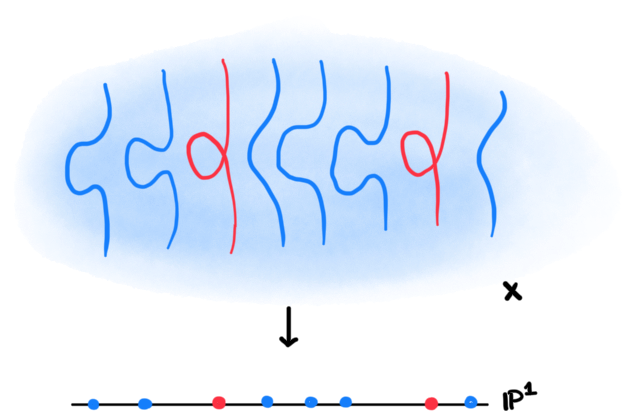
\includegraphics[width=0.7\textwidth]{images/Sketch 12.png}
\end{center}
Deleting the singular fibers, we obtain a locally trivial fibration by
Ehresmann's lemma and hence we have
\[
   \sum_{C \text{ a singular fiber}} \chi_\textnormal{top}(C)=
   \chi_\textnormal{top}(X) = 24.
\]
But singular fibers in this case are rational, hence \(X\) has at least 24
rational curves (for simplicity, we assume all curves are reduced, irreducible,
and at worst nodal.)

Likewise, if \(h=2\) then the map \(X\to \mathbb{P}^2\) is a double cover
branched over a sextic curve \(C\subset \mathbb{P}^2\). Such a curve has \(324\)
bitangent lines, each of which pulls back to a fiber with two nodes (again
rational, since a generic fiber has genus \(2\)). If \(h=3\), \(X\into
\mathbb{P}^3\) is a quartic hypersurface and the rational elements in the linear
system come from tri-tangent planes like we discussed before. There are
precisely \(3200\) such planes.

\subsection{The Yau--Zaslow formula} Write \(N_{0,h}\) for the count of genus
\(0\) curves in the linear system associated to a general algebraic K3 surface.
The data of \(h\) fixes a cohomology class \(\beta\in
\Pic(X)=\HH^2(X,\mathbb{Z})\cap \HH^{1,1}(X)\) with \(\beta^2=2h-2\), and we
are counting (stable) curves \(\mathbb{P}^1\to X\) with image in this
cohomology class. From the above discussion, the first few values of \(N_{0,h}\)
are \(24,324,3200,\ldots\). Yau and Zaslow spotted that these coincide with the
coefficients of a well-known modular form, and conjectured the following.

\begin{theorem}[(Yau--Zaslow formula)]
    Writing \(\Delta(z)=(\prod_{n\geq 1}(1-z^n)^{24})^{-1}\) for the
    discriminant modular form, we have the identity
    \[
        \sum_{h\geq 0}N_{0,h}\cdot z^h = \frac{z}{\Delta(z)}=1+24z+324z^2+\cdots
    \]
\end{theorem}

This was proven independently Beauville and Bryan--Leung. How might one prove
this? Inspired by the construction for \(h=1\), we will build
another fibration. The base is the linear system \(\mathbb{P}^h\), and the total
space is the compactified Jacobian of the universal curve \(\mathscr{C}\into
\mathbb{P}^h\) i.e.\ the fiber over a smooth curve \(C\in \mathbb{P}^h\) is the
Jacobian \(\Jac(C)\). The space is compactified to include nodal fibers, via a
generalised Jacobian construction (for \(h=1\) this is the same fibration we
had, since an elliptic curve is its own Jacobian.)

Now the Jacobian \(\Jac(C)\) has trivial Euler characteristic if \(C\) is smooth
or has genuine genus (eg. the first two fibers in the picture), while
\(\chi_\text{top}(\Jac C)=1\) if \(C\) is rational. Thus we have
\[N_{0,h}=\sum_{\text{rational curves \(C\)}}\chi_\text{top}(\Jac
C)=\chi_\text{top}(\overline{\Jac}(\mathscr{C}/\mathbb{P}^h)).\]

\begin{center}
    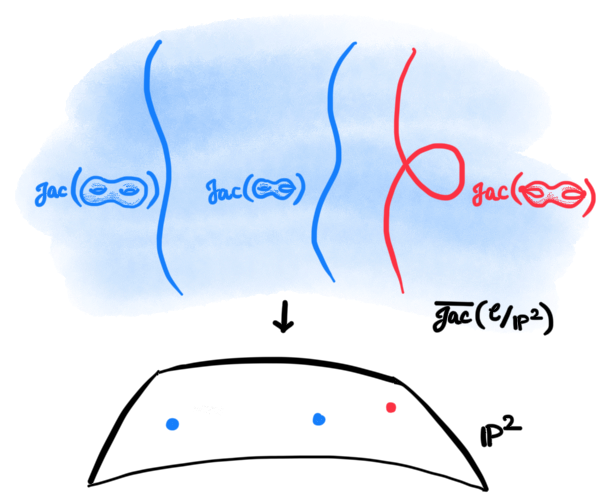
\includegraphics[width=0.7\textwidth]{images/Sketch 13.png}
\end{center}
Moreover, by a result of Huybrechts we have that
\(\overline{\Jac}(\mathscr{C}/\mathbb{P}^h)\) is birational to the Hilbert
scheme \(\text{Hilb}^h (X)\), and the Euler characteristic of the latter has
been computed by G\"ottsche as the coefficient of \(z^h\) in
\(\frac{z}{\Delta(z)}\). A result of Batyrev--Kontsevich shows that two
birational Calabi--Yau manifolds have the same Betti numbers, which concludes
our argument.

\section{Introduction to Gromov--Witten theory}
The way we computed the counts on a K3 surface exploited the specific geometry
in the situation. We will now describe a more general framework for counting
curves, which involves two steps. First, we build a moduli space of curves in
\(X\) of a fixed type (genus, cohomology class) --- if this has dimension zero
then we obtain an honest count, otherwise we impose natural conditions by doing
intersection theory on this moduli space.

\begin{example}
    There are infinitely many conics (i.e.\ rational curves of degree \(2\)) in
    \(\mathbb{P}^2\). These are parametrised by the moduli space
    \(\Moduli_{0,2}\mathbb{P}^2=\mathbb{P}^5\), since a conic is determined by a
    degree \(2\) homogeneous polynomial in three variables. Thus to obtain a
    count, we may impose the condition that our curve passes through five fixed
    points \(\{p_1,\ldots,p_5\}\). Each point gives a linear constraint, and hence
    if the five points are in general position then there is a unique conic
    passing through them (corresponding to the intersection of the five general
    hyperplanes.)
\end{example}

As a general principle, the count should not depend on the specific choice of
points. To make this rigorous, we replace each hyperplane \(H_i=\{\text{conics
through \(p_i\)}\}\) with its (Chow) homology class \([H_i]\), and then define
the intersection to be given by cup products of Poincar\'e duals
\[[H_1]\cdot \ldots\cdot [H_5]=\int_{[\mathbb{P}^5]}\textnormal{PD}[H_1]\cup \ldots
\cup \textnormal{PD}[H_5] = 1.\]
The count then depends only on the cohomology classes of the constraints.
Theories of modern enumerative geometry follow this principle.

\begin{remark}
    In general, there are two to think about curves in \(X\) --- via
    parametrisations (i.e.\ as maps \(C\to X\)), or via equations. Thus for
    curves in \(\mathbb{P}^2\) one might think of parametrisations
    \([z:w]\mapsto [z^2:zw:w^2]\) or equations \(\mathbb{V}(xz-y^2)\). The first
    approach leads to Gromov--Witten theory, while the latter gives rise to
    Donaldson--Thomas theory.
\end{remark}

Thus to do Gromov--Witten theory, we first fix a genus \(g\geq 0\) and a
cohomology class \(\beta \in \HH^2(X,\mathbb{Z})\), and `guess' the moduli space
\[
    \Moduli_g(X,\beta)=\{C\xrightarrow{f} X\;|\; C\text{ a smooth curve of
    genus \(g\),} \quad f_\ast[C]=\beta\}.
\]
However, this na\"ive moduli space is often non-compact (and hence unsuitable
for intersection theory.) To get a compactification, we have to allow maps \(f\)
from nodal curves which may contract components. The well-behaved maps of this
kind are called stable (defined later). Our space of interest, now compact,
is
\[
    \overline{\Moduli}_g(X,\beta)=\{C\xrightarrow{f}X\;|\; C\text{ an at worst
    nodal curve of genus \(g\)}, \quad f\text{ stable,}\quad f_\ast[C]=\beta\}.
\]
To impose constraints, it is also often convenient to consider curves with
\(n\geq 0\) \textit{marked points} \(p_1,\ldots,p_n\in C\), and form the moduli
space \(\overline{\Moduli}_{g,n}(X,\beta)\) of stable maps \(f:C\to X\) with
prescribed behaviour (e.g.\ tangency conditions) at \(f(p_i)\).

\begin{definition}
    Let \(C\) be a nodal curve of genus \(g\) with \(n\) marked points. A
    map \(f:C\to X\) is \textit{stable} if every rational component contracted
    by \(f\) has at least three nodes or marked points, and every contracted
    elliptic component has at least one node or marked point.
\end{definition}

\begin{center}
    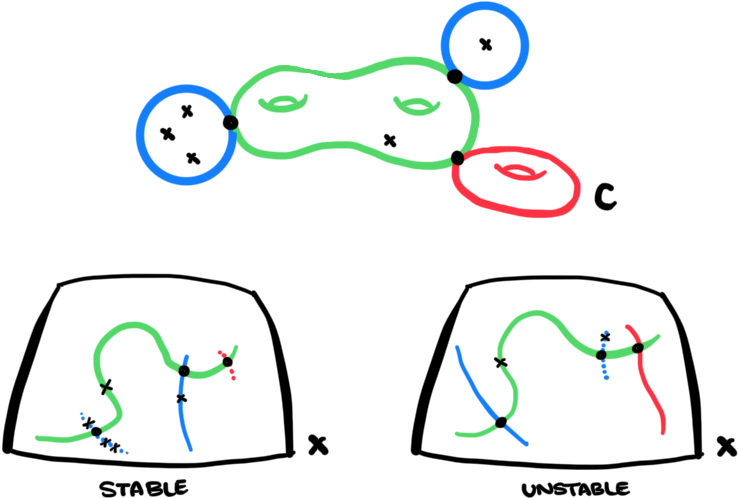
\includegraphics[width=0.5\textwidth]{images/Sketch 14.png}
\end{center}

We have succeeded, by obtaining a compact moduli space
\(\overline{\Moduli}_{g,n}(X,\beta)\). At what cost? We have added way more junk
--- the
complement \(\overline{\Moduli}_{g,n}(X,\beta)\setminus \Moduli_{g,n}(X,\beta)\)
is often massive and has components of dimension (way) higher than the original
space. To make matters worse, \(\overline{\Moduli}_{g,n}(X,\beta)\) often does
not have a fundamental class --- we have nothing to integrate over for
intersection theory!

The second of these problems is remedied by introducing a \textit{virtual
fundamental class} \([\overline{\Moduli}_{g,n}(X,\beta)]^\textnormal{vir}\), if
we are lucky this coincides with the fundamental class (this happens, for
instance, for \(\overline{\Moduli}_{0,n}(\mathbb{P}^N, d)\). If not, we pretend
the compactified moduli space of interest \(\Moduli\) is cut out by \(r\)
equations in a smooth ambient space \(Y\) of dimension \(N\). The excess junk of
dimension \(>N-r\) arises precisely because the intersection is not transverse
in places, so we perturb these equations to make it transverse and think of
\([\Moduli]^\textnormal{vir}\in \HH_{N-r}(\Moduli)\) as the fundamental class of
this perturbed space.

\begin{minipage}[c]{0.6\textwidth}
\begin{example}
    Suppose \(\Moduli=\mathbb{V}(xz,yz)\subset \mathbb{P}^3\) is the union of a
    line \(L=\mathbb{V}(x,y)\) (the space of interest) and a plane
    \(\mathbb{V}(z)\) (the junk). Perturbing the
    equations, we obtain \(\mathbb{V}(xz-\epsilon y^2, yz-\epsilon xw)\) which
    is the union of the line \(L\) and a twisted cubic
    \(C_\epsilon:[u,v]\mapsto (v^3,\epsilon uv^2, \epsilon^2 u^2v, \epsilon^3
    u^3)\). In the limit, we have a plane cubic \(C_0\subset \mathbb{V}(z)\) and
    the virtual fundamental class of \(\Moduli\) is
    \([\Moduli]^\text{vir}=[L]+[C_0]\).
\end{example}
\end{minipage}\hspace{0.03\textwidth}
\begin{minipage}[c]{0.4\textwidth}
        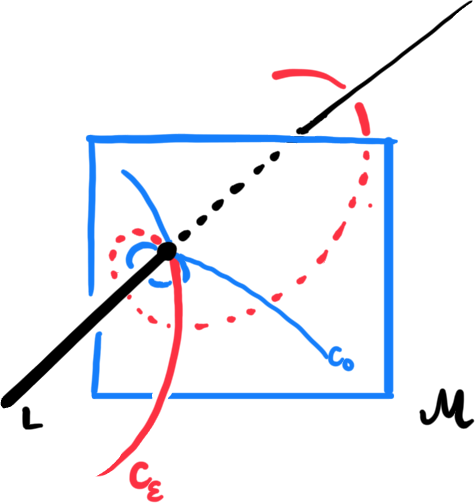
\includegraphics[width=0.6\textwidth]{images/Sketch 15.png}
\end{minipage}


Then the \textit{Gromov--Witten invariants} are defined as integrals of the form
\(
    \int_{[\overline{\Moduli}_{g,n}(X,\beta)]^\textnormal{vir}}[\textnormal{constraints}]
\)
where the constraints usually naturally arise from the setting of the problem
and live in the same dimension as the virtual fundamental class. Because the
moduli space has so much junk and the fundamental class is virtual, these are
not really curve counts any more. However, they are better behaved in other
ways --- they are deformation invariant, and naturally arise in mirror symmetry.
And often, they do help compute actual curve counts.

\subsection{Gromov--Witten theory of a K3 surface}
Let \(X\) be a K3 surface and \(\beta\in \Pic X\) a primitive class with
\(\beta^2=2h-2\). Rather annoyingly, the virtual fundamental class
\([\overline{\Moduli}_g(X,\beta)]^\textnormal{vir}\) is zero for all \(g\). This
is related to the ``\(-1\)'' dimension count we obtained earlier, though we do
not go into the details. The fix here is to define a `reduced virtual
fundamental class' \([\overline{\Moduli}_g(X,\beta)]^\textnormal{red}\), which
is non-zero and lives in \(\HH_g(\overline{\Moduli}_g(X,\beta))\). In particular
for rational curves this class has degree zero, and the curve counts are simply
\[
    N_{0,h}= \int_{[\overline{\Moduli}_g(X,\beta)]^\textnormal{red}}1.
\]
For \(g>0\) the curve count is infinite, since the virtual dimension of the
moduli space is positive. To get a finite number, we impose a
\(g\)-dimensional condition \(\lambda_g\) to obtain a count
\(N_{g,h}\) (this condition is vacuous for \(g=0\).) Roughly speaking, this
condition arises from a rank \(g\) vector bundle \(\mathbb{E}_g\to
\overline{\Moduli}_g(X,\beta)\) whose fiber over a stable curve \(C\) is given
by \(\HH^0(C,\omega_C)\). Thus these constraints are sufficiently natural, and
we get meaningful invariants of \(X\).

The Yau--Zaslow formula has a generalisation in higher genera, called the KKV
conjecture. This asserts that generating series for \(N_{g,h}\) lie in the ring
of quasi-modular forms, and was proven by Maulik, Pandharipande, and Thomas.

\section{Logarithmic Gromov--Witten theory}

To see how marked points play a role in Gromov--Witten theory, we will now try
to answer questions of the flavour `how many (stable) curves of fixed type in a
variety \(X\) have prescribed tangency conditions to a given divisor
\(D\subset X\) with  simple normal
crossings?' Concretely, let us count degree \(d\) plane rational curves that are
maximally tangent to each axis. Thus we are looking at degree \(d\) maps
\(f:\mathbb{P}^1\to \mathbb{P}^2\) such that \(f(\mathbb{P}^1)\cap
\mathbb{V}(x)=d\cdot f[0:1]\) and likewise for the other markings.
\begin{center}
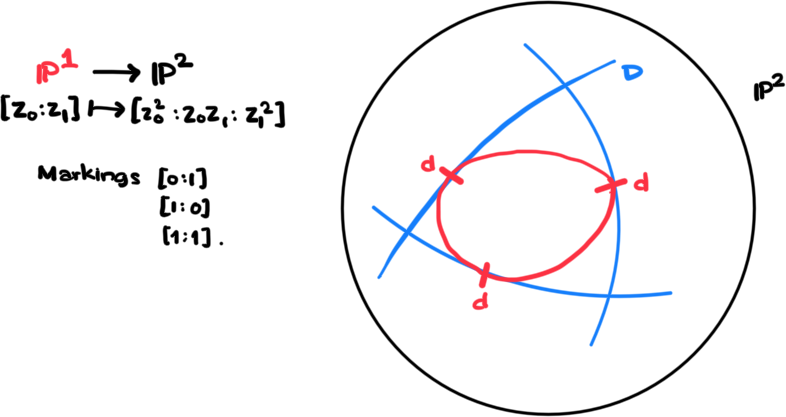
\includegraphics[width=0.6\textwidth]{images/Sketch.png}
\end{center}

In general, we fix \(g,n,\beta\) as before and \(\alpha\) a collection of
integers giving the desired tangency of the \(i\)th marking to \(D\). Consider the moduli space
\[
    \Moduli_{g,\alpha}(X|D, \beta) = \left\{ \text{smooth curves
}C\xrightarrow{f}X \text{ of genus \(g\)  and degree \(\beta\) with tangency
\(\alpha\) with \(D\)}\right\}.
\]
Is this compact? No --- as before, we have only allowed smooth curves so we fix
that by asking for stable nodal curves instead. The resulting space is still
non-compact, because it does not include curves that degenerate into \(D\). For
example, consider the curve given by \([z_0:z_1:t(z_0-z_1)]\) as \(t\rightarrow
0\). In the limit, the curve degenerates into \(D\) as shown below.

\begin{center}
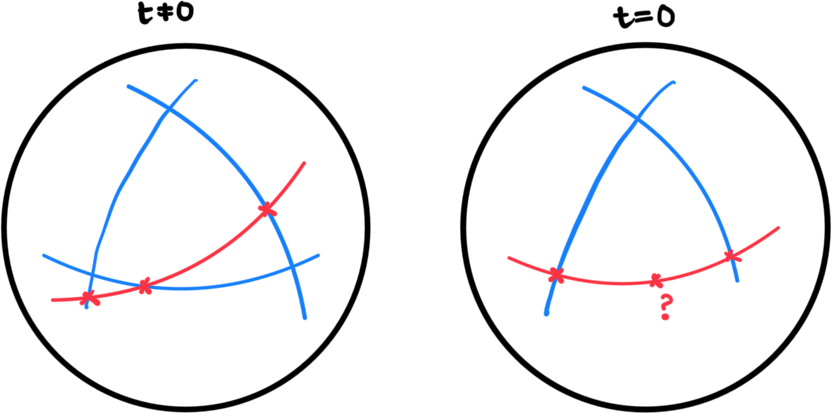
\includegraphics[width=0.6\textwidth]{images/Sketch 2.png}
\end{center}

Thus we need a new fix for this problem. For this, we will need to think
torically/tropically, by `discretising' each of the players \(X,C,f\) in the
problem.

\subsection{The tropicalisation game} In general, we follow the following rules:
the pair \(X,D\) is replaced by the associated toric fan, and the curve \(C\)
becomes a graph with vertices representing irreducible components, edges
representing nodes, and `floating' edges corresponding to other markings.

\begin{center}
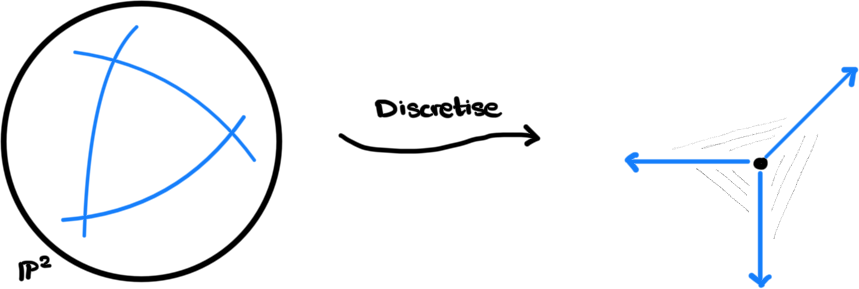
\includegraphics[width=0.35\textwidth]{images/Sketch 3.png} \qquad \qquad
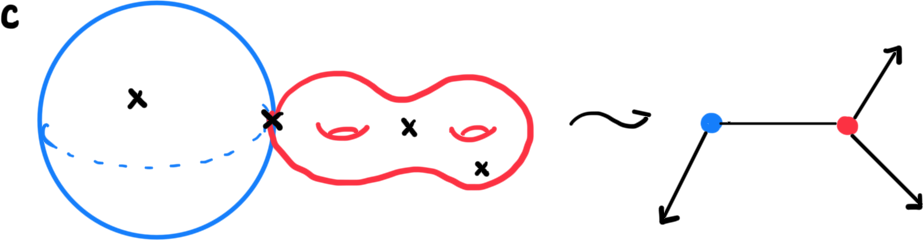
\includegraphics[width=0.35\textwidth]{images/Sketch 4.png}
\end{center}

The map \(f:C\to X\) is then represented by a linear embedding of the graph,
where each vertex maps into the cone of the toric stratum in which the curve
generically sits. The floating edges are parallel to the ray which gives the
component of \(D\) on which the corresponding marked point lies.

\begin{center}
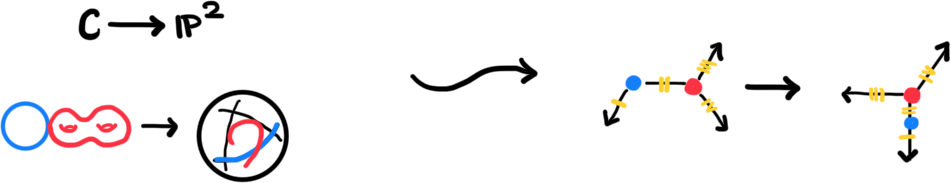
\includegraphics[width=0.8\textwidth]{images/Sketch 5.png}
\end{center}

Thus for the family of curves \([z_0:z_1:t(z_0-z_1)]\), we have
\begin{center}
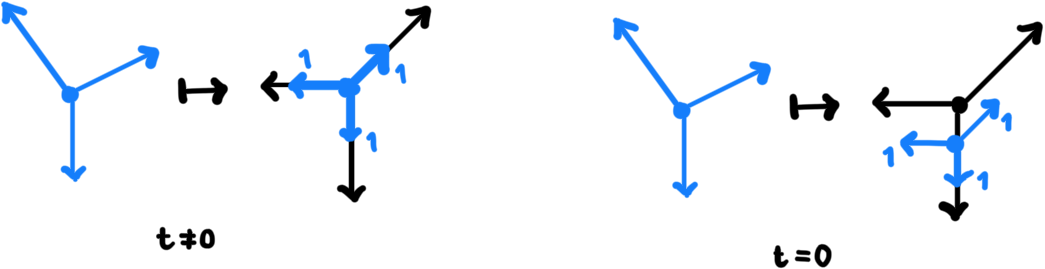
\includegraphics[width=0.7\textwidth]{images/Sketch 16.png}
\end{center}

\subsection{What's in the moduli space?} Say vertex in the degenerated curve is
\textit{balanced} if the sum of all outgoing vectors is zero. To first
approximation, we add into our moduli space those stable maps whose
discretisation is balanced. For example, the following map is detected. \begin{center}
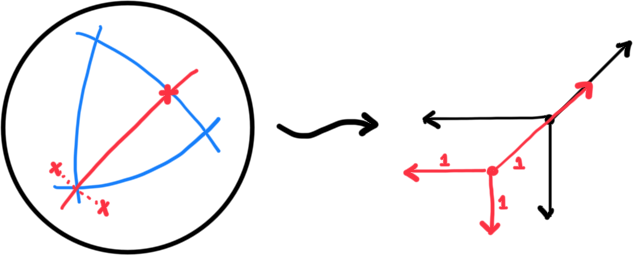
\includegraphics[width=0.5\textwidth]{images/Sketch 7.png}
\end{center}

The resulting space \(\overline{\Moduli}^{\text{log}}_{g,\alpha}(X|D,
\beta)\supset \mathcal{M}_{g,\alpha}(X|D,\beta)\) is compact, and is called the
\textit{moduli space of stable logarithmic maps}. This, as before, does not have
a fundamental class but does have a virtual one. Doing intersection theory on
the space then gives \textit{logarithmic Gromov--Witten invariants}.

\subsection{Curve counts using log Gromov--Witten theory} To count general
curves (and hence bring log Gromov--Witten theory closer to the ordinary one),
we can enforce generic tangency conditions with the divisor. For example, a
general degree \(d\) curve in \(\mathbb{P}^2\) looks like
\begin{center}
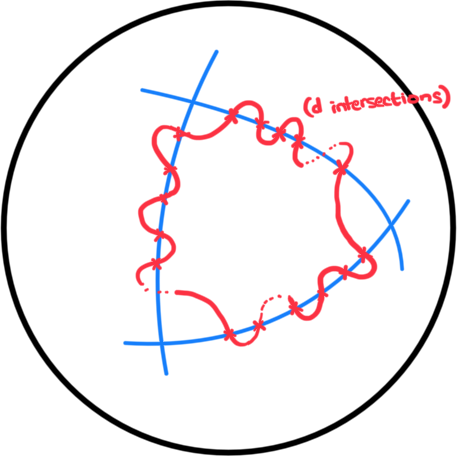
\includegraphics[width=0.3\textwidth]{images/Sketch 8.png}
\end{center}
so we impose a generic tangency constraint by considering \(\mathbb{P}^1\) with
\(3d\) marked points. This gives a \(3d-1\) dimensional space of generic degree
\(d\) curves, so by imposing additional conditions (e.g.\ requiring the curve to
pass through \(3d-1\) fixed points \(p_1,\ldots,p_{3d-1}\in \mathbb{P}^2\)) we can
define the Gromov--Witten invariant
\[
    N^{\mathbb{P}^2}_{0,d}=\int_{[\overline{\Moduli}_{0,\alpha}(\mathbb{P}^2|D,
    d)]^\text{vir}}[\text{condition to pass through }p_1,\ldots,p_{3d-1}].
\]
It turns out the problem is sufficiently nice and this is equal to the number of
rational degree \(d\) curves in \(\mathbb{P}^2\) through \(3d-1\) generic
points. Moreover, it can be computed combinatorially by using the the following
theorem and other similar results.

\begin{theorem}[(Mikhalkin)]
    The number \(N_{0,d}^{\mathbb{P}^2}\) is equal to the number of
    ``discretised curves'' in the toric fan of \(\mathbb{P}^2\)  with \(d\)
    unbounded arrows in each divisorial direction, and passing through through
    \(3d-1\) points in \(\mathbb{R}^2\).
\end{theorem}

\begin{minipage}[c]{0.6\textwidth}
Thus for example if \(d=1\), there is a unique balanced curve passing through
two points fixed points in \(\mathbb{R}^2\) with balanced vertices and one
unbounded arrow in each direction. This, of course, corresponds to the fact that
there is a unique rational curve through two fixed points in \(\mathbb{P}^2\).
\end{minipage}\hspace{0.03\textwidth}
\begin{minipage}[c]{0.4\textwidth}
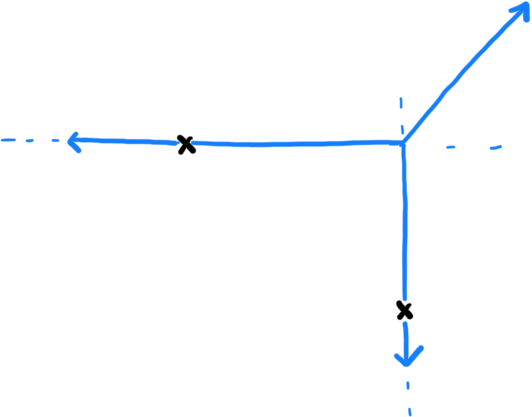
\includegraphics[width=0.7\textwidth]{images/Sketch 9.png}
\end{minipage}

\section{Counts in higher genus}
We have seen that generalised counts of rational curves (i.e.\ Gromov--Witten
invariants for genus \(0\)) on \(\mathbb{P}^2\) are related to tropical
curve counts. We will now see how this generalises to statements about higher
genus curves. In general forming a logarithmic moduli space of higher genus
curves is hard, so we first rephrase the genus \(0\) problem in purely tropical
terms.

Recall the goal was to measure
\(N_{0,d}^{\mathbb{P}^2}=\#\{\text{plane rational curves of degree \(d\) through
\(3d-1\) points}\}\), and we did this by defining a combinatorial gadget. We
make this precise. 

For this, fix the data
\(\Delta_d=\{(-1,0),\overset{d}{\ldots},(-1,0),(0,-1),\overset{d}{\ldots},(0,-1),(1,1),\overset{d}{\ldots},(1,1)\}\).

\begin{definition}
     A \textit{rational tropical curve of degree \(\Delta_d\)} is given by
    \begin{enumerate}[(i)]
        \item a graph \(\Gamma\) of genus zero with vertices, bounded edges, and
            \(3d\) unbounded edges,
        \item a real number for each bounded edge called the length, and
        \item a map \(h:\Gamma \to \mathbb{R}^2\) such that each unbounded edge
            is parallel to the corresponding vector in \(\Delta_d\) and the
            bounded edges are mapped to segments of the specified length, and
            the sum of outgoing edges at each vertex is zero.
    \end{enumerate}
\end{definition}

Then Milkhalkin shows that \(N^{\mathbb{P}^2}_{0,d}\) is equal to the number
of (weighted) rational tropical curves of degree \(\Delta_d\) through \(3d-1\) points.  Thus for example, if \(d=2\) then five points determine a unique conic as shown.
\begin{center}
    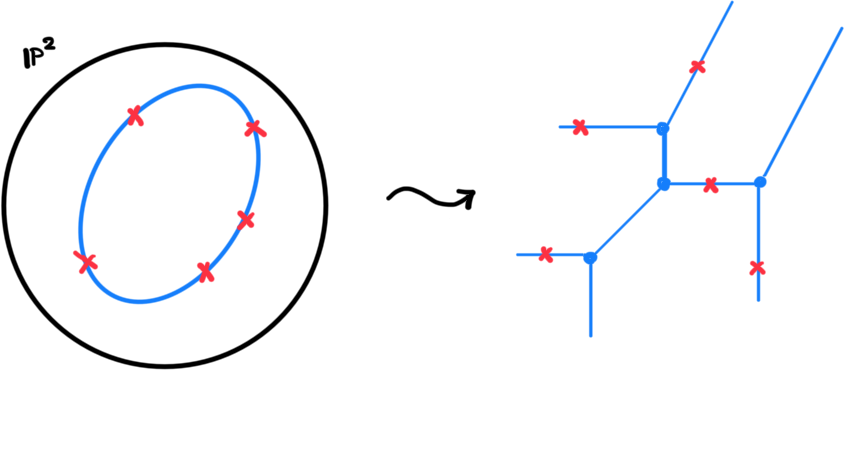
\includegraphics[width=0.6\textwidth]{images/Sketch 10.png}
\end{center}

\subsection{Why should you be able to relate curve counts to tropical curves?}
Of course we know that \(N_{0,d}^{\mathbb{P}^2}\) is secretly a logarithmic
Gromov--Witten invariant and in the logarithmic moduli space, this
tropicalisation procedure produces tropical curves. The principle at play here
is that invariants of a space should be related to those of its degenerations,
which are precisely encoded by tropical curves.
\begin{center}
    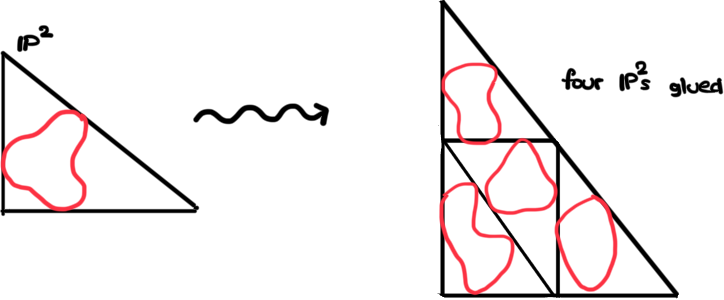
\includegraphics[width=0.5\textwidth]{images/Sketch 11.png}
\end{center}
Then the curve count we require can be computed from the counts in each segment,
and these correspond to multiplicity of the vertices of the tropical curve.

\subsection{Higher genus tropical curves} Thus to compute log Gromov--Witten
invariants for positive genus, we begin by asking what a higher genus
generalisation of tropical curve would be. The answer comes from examining the
higher genus case of K3 surfaces, which was solved earlier.

For K3 surfaces, G\"ottsche and Shende produce series \(N_{0,h}(q)\) that
evaluates the invariant \(N_{0,h}\) at \(q=1\). Combining this with
Maulik--Pandharipande--Thomas' solution to the KKV conjecture, we have the
identity
\[
    \sum_{g\geq 0}N_{g,h}u^{2g-2} =
    (-1)(q^\frac{1}{2}-q^{-\frac{1}{2}})^{-2}N_{0,h}(q) \qquad \text{ at }q=e^{iu},
\]
i.e.\ higher genus counts \(N_{g,h}\) are computed by a series
\(N_{0,h}(q)\).

But G\"ottsche and Shende also give a very similar series
\(N_{0,d}^{\mathbb{P}^2}(q)\), so mimicking the above formula we guess that
there are higher genus tropical curve counts \(N_{g,d}^{\mathbb{P}^2}\) satisfying
\[
    \sum_{g\geq 0}N_{g,d}^{\mathbb{P}^2}u^{2g-2+3d} =
    (i(q^\frac{1}{2}-q^{-\frac{1}{2}}))^{3d-2}N_{0,d}(q) \qquad\text{ at }q=e^{iu}.
\]
Bousseau was able to give a precise definition of higher genus
invariant \(N_{g,d}^{\mathbb{P}^2}\) with an appropriate ``\(\lambda_g\)
condition'' such that the above formula holds. Moreover in analogy with the
K3 case, analogous to the K3 case, these invariants are related to higher genus
tropical curve counts with refined multiplicity. The details of this are beyond
the scope of these lectures.
